\documentclass[conference]{IEEEtran}
\IEEEoverridecommandlockouts
% The preceding line is only needed to identify funding in the first footnote. If that is unneeded, please comment it out.
\usepackage{cite}
\usepackage{amsmath,amssymb,amsfonts}
\usepackage{algorithmic}
\usepackage{graphicx}
\usepackage{textcomp}
\usepackage{xcolor}


\newcommand{\ex}[1]{x^{(#1)}}
\newcommand{\es}[1]{s^{(#1)}}
\newcommand{\ey}[1]{y^{(#1)}}


\begin{document}

\title{Deep Learning Methods to Help Predict Properties of Molecules from SMILES}

\author{\IEEEauthorblockN{Manuel Rodriguez-Martinez}
\IEEEauthorblockA{\textit{Department of Computer Science and Engieering} \\
\textit{University of Puerto Rico, Mayag\"{u}ez}\\
Mayag\"{u}ez, PR \\
manuel.rodriguez7@upr.edu}
\and
\IEEEauthorblockN{Gretchen Bonilla-Caraballo}
\IEEEauthorblockA{\textit{Department of Computer Science and Engieering} \\
\textit{University of Puerto Rico, Mayag\"{u}ez}\\
Mayag\"{u}ez, PR \\
gretchen.bonilla@upr.edu}
}
\maketitle

\begin{abstract}
Last part to do.
\end{abstract}

\begin{IEEEkeywords}
Deep Learning, SMILES, PubChem
\end{IEEEkeywords}

\section{Introduction \label{intro}}

\subsection{Contributions}
\subsection{Paper Organization}
The rest of this paper is organized as follows. In section \ref{background} we provide background and motivation material to set the context for the remainder of the paper. In section \ref{archi} our deep learning models that can be used to help predict properties of molecules, using SMILES representations. Our experimental setup and results are presented in section \ref{experiments}. Related works are presented and discussed in section \ref{relwork}. Finally, section \ref{conclude} contains our summary of results, conclusions, and future works.

\section{Motivation and Background  \label{background}}
\subsection{Motivation}
As we mentioned in the section \ref{intro}, a key goal of our efforts  is to develop methods to use DL to help predict properties of molecules from first principles. That is, rather than trying to engage in complex and often {\em intuition-based} feature engineering efforts that require experienced domain scientists, we want to use basic and readily available chemical and physical information as input to the models. The rationale behind this is that deep neural networks have been shown to excel at using early layers in the network as {\em feature generators} that are then used by mid and late layers in the network. Properly trained and tuned deep models have been shown to rival or surpass  human ability in domains such as language translation and computer vision (REFS). Thus, a successfully trained model that is based on first principle data can help a wider range of scientists and practitioners study and predict properties of novel molecules. 

Publicly available databases, such as PubChem (REF) and OQMD (REF) provide the foundational information from which to draw the set of basic features to serve as input  to the model. These databases provide a) chemical properties, b) physical properties, c) 2D and 3D imaging on spatial structures of molecules,  and d) 2D imaging on molecular spectroscopy, to name a few.

\subsection{Problem Formulation}
We can state our problem as follows. Supposed we have a data set $\mathcal{S}$, consisting of a collection of records $s_0, s_1, ..., s_n$ containing information about some group of molecules. Let $\mathcal{P} = \{p_0, p_1, ..., p_r\}$ be a collection of molecular properties that we want to predict or estimate from $\mathcal{S}$.  Our task is to: 
\begin{enumerate}
	\item Transform $\mathcal{S}$ into an input data set $X = \{x_0, x_1, ..., x_m\}$, where each element $x_i$ is an example that represents 
	some set of properties extracted from an item $s_j \in  \mathcal{S}$. In this case, each example $x_i$ is a multi-dimensional vector and 
	$X$ is a matrix containing these examples.
	\item Define one or more deep learning models $M_0, M_1, ... M_p$ that predict the properties in $\mathcal{P}$. Thus, the prediction $y$ for a given model $M_k$ might contain one or more of the properties in $P$. In other words, in theory, the prediction $y$ can be a multi-dimensional vector $y = \{y_0, y_1, ..., y_l\}$ , $l \leq r$, where each component represents some property in $\mathcal{P}$. For simplicity, in this paper we only consider models that predict one property at time,  from the input data $X$. Hence the model's output is one-dimensional
	\item Use $X$ to train one or more deep learning models $M_0, M_1, ... M_p$. For each $x_i$ in $X$, a given model $M_k$ will output a prediction $y_i$. The collection of predictions $y_0, y_1, ..., y_m$ forms a column vector $Y$. 
\end{enumerate}
Thus, we have established the basic framework to handle the task of molecular property prediction as a regular machine learning problem. 
\subsection{PubChem Database}
The PubChem\footnote{PubChem URL: https://pubchem.ncbi.nlm.nih.gov} Database is one of the largest databases of chemical molecules and their properties. PubChem is freely available and is maintained by the National Library of the Medicine of the U.S. National Institutes of the Health (NIH). The database contains hundreds of millions of entries and provide search capabilities based on the name of the chemical, its molecular formular, or its compound identifier.  Programatic access to  PubChem is available through PUG-REST (REF), a Python-based REST API. 

For the purpose of this paper, we shall focus on a sub-set of PubChem that contains the following basic molecular properties:
\begin{enumerate}
	\item {\em CID} - unique compound identifier within PubChem. This a nine-digit numeric string. 
	\item {\em Molecular Formula} -  a string that specifies the type and number of atoms in a molecule. For example, the molecular formula for the widely-used analgesic acetaminophen is C8H9NO2.
	\item {\em Canonical SMILES} - a string that specifies the chemical structures and bonds in a molecule. For example, the Canonical SMILES string for acetaminophen is CC(=O)NC1=CC=C(C=C1)O. We shall discuss more about the SMILES notation is section \ref{smiles}.
	\item {\em Isomeric SMILES} - a variation of the SMILES notation that includes isomers - molecules with identical molecular formula but different arrangement of its constituents atoms in space. The Isomeric SMILES for acetaminophen is [2H]C1=C(C(=C(C(=C1NC(=O)C)[2H])[2H])O)[2H].
	\item {\em Molecular Weight} - this is real number that represents the mass of a given molecule and its measured in {\em daltons}, or in molar mass (g/mol). The molecular weight for acetaminophen is 155.19 g/mol.
	\item {\em XLogP} - this is real number representing the logarithm of the partition coefficient $\boldsymbol P$ of the molecule with respect to 1-octanol and water, and computed with the XLogP3 method. 
\end{enumerate}
PubChem has many more data elements, and we encourage the interested reader to further explore this comprehensive database. 

\subsection{SMILES Representations\label{smiles}}
The Simplified Molecular Input Line Entry System (SMILES) is a character-based line notation for describing chemical structures in a way that is easier for computers to interpret. SMILES strings can be mapped into two-dimensional or three-dimensional models of the spatial organization of the atoms in the molecules being represented by the string. The notation consists of a series of characters containing no spaces that uses a simple vocabulary and a few grammar rules. In this notation atoms are represented by their atomic symbol while bonds and branches are represented by special characters.

One complication with SMILES is that straightforward application of the basic rules for generating a SMILES string can yield more than one string representation per molecule. To solve this, some {\em canonicalization} algorithm is typically used in chemical databases to  assign just one representation per structure and permit consistency. In PubChem, this representation is called {\em Canonical SMILES}. 
{\em Isomeric SMILES} are a variation of SMILES in which information on isotopes and stereochemistry (i.e., 3-D structures) is included within the string. A detailed description of the specifics of these canonicalization algorithms, isomeric variations, and stereochemistry is beyond the scope of this paper (REF). 
%
%    \begin{itemize}
%        \item Simplified Molecular Input Line Entry System (SMILES) is a line notation for describing chemical structures in a way that is easier for computers to interpret. 
%        \item It consists of a series of characters containing no spaces that uses a simple vocabulary and a few grammar rules.
%        \item In this notation atoms are represented by their atomic symbol while bonds and branches are represented by special characters.
%        \item Unfortunately based exclusively on the basic rules for generating a SMILES string there can exist more than one way to represent a single compound.
%        \item To help assign just one representation per structure and permit consistency a canonicalization algorithm is typically used by databases. This algorithm's job is to generate and assign one specific SMILES string for each structure.
%        \item In our dataset these are called canonical SMILES.
%        \item Another type of SMILES string that are often used and are also available in our dataset are isometric SMILES. These include isotopic specifications of a chemical structure.
%    \end{itemize}
    \subsubsection{SMILES Rules}
        \begin{enumerate}
            \item Atoms are represented by their atomic symbol and are enclosed in brackets []. The organic subset can be written without brackets, these include: B, C, N, O, S, F, Cl, Br, and I. Brackets can also be used to remove ambiguities about the charge of the atom. 
            \item Bonds are represented as follows:
            \begin{itemize}
                \item[$-$] single bond
                \item[$=$] double bond
                \item[$\#$] triple bond
                \item[$.$] disconnected structure
            \end{itemize}
            \textbf{Note:} Single bonds can be omitted as shown in Figures \ref{fig:smile-examples} and \ref{fig:smile-examples2}.
            \item Branches are represented with parenthesis, ().
            \item Cyclic structures or carbon rings are represented with digits. The first digit is the beginning of the rings and the matching digit that follows is when the ring closes. This can also be observed in Figures \ref{fig:smile-examples} and \ref{fig:smile-examples2}.
        \end{enumerate}
    \subsubsection{Correspondence between the 2D structure and a SMILES}
        \begin{itemize}
            \item In Figure \ref{fig:smile-examples} we can see two chemical models each with a cyclic cycle.
            \item Each edge and end of the 2D model represent a carbon and in both the model and SMILES the hydrogen is omitted as it is assumed that they fill any missing bonds.
            \item Notice in Figure \ref{fig:smile-examples} the leftmost figure its SMILES has a double bond which is illustrated in the 2D model. It is then followed by a digit indicating that the next sequence is for a cyclic structure. 
            \item So in this first figure we have that it starts at a carbon which is the starting point for a cyclic cycle and the cycle starts with a double bond. 
            \item In the rightmost image we see similarly that it starts with a carbon, in this case it is the one located at the leftmost edge of the triangle. This carbon starts the cycle that includes an oxygen atom and note that when the cycle closes the next part of the SMILES continues from the initial carbon.
            \item In Figure \ref{fig:smile-examples2} we can observe a more detailed example that better illustrates how the various rules come together to represent what we see in the 2D model.
            \item The initial red 'C' in the SMILES is shown in the 2D structure with the red circle. That is our starting position. 
            \item This is followed by a '1' implying that the red 'C' belongs in a carbon ring and will be treated as the starting point of it. And the carbon ring closes at the orange 'C' since this is followed by the second '1'.
            \item We can notice as well that the orange 'C' also forms part of a branch as it is enclosed in a parenthesis. The entire branch can be observed in the 2D model inside the purple circle.
            \item Finally the green text of the SMILES can be seen inside the green circle. Notice that it is attached to the first carbon of the SMILES (red 'C'). 
        \end{itemize}
    
    \begin{figure}[h]
        \centering
        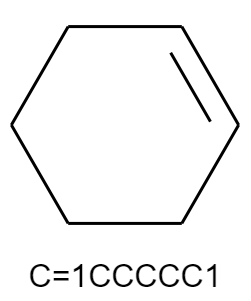
\includegraphics[width=0.25\textwidth]{figures/Smiles-Smile1.png}
        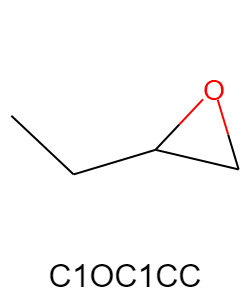
\includegraphics[width=0.25\textwidth]{figures/Smiles-Smile2.png}
        \caption{Example of 2 chemical structures and their respective SMILES}
        \label{fig:smile-examples}
    \end{figure}
    \begin{figure}[h]
        \centering
        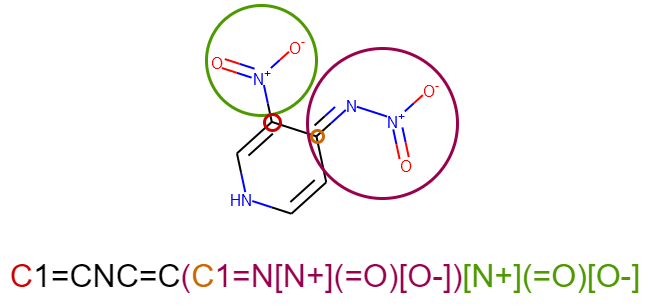
\includegraphics[width=0.5\textwidth]{figures/Smiles-Smile3.png}
        \caption{Example of how each part of the SMILES string corresponds to the 2D model of the chemical structure.}
        \label{fig:smile-examples2}
    \end{figure}
\subsection{Applying NLP Ideas}




\section{Deep Learning Architectures \label{archi}}
    % Model descriptions
    \subsection{Deep Learning to Predict Molecular Weight from SMILES}
        \begin{itemize}
            \item The first model we will discuss is a DL model that receives an embedded SMILES string as input and as a result returns its prediction of the molecular weight. This model is shown in Fig.\ref{fig:mw-architecture}.
            \item Its architecture consisted first of a character embedding layer, that initially had random weights.
            \item This layer receives the pre-processed SMILES strings as input.
            \item Its output is then passed to a 1D Convolutional Neural Network (CNN) and is later flattened.
            \item This is followed with a fully connected layer that connects to a dropout layer.
            \item Finally, it ends with a 1 neuron dense layer that outputs the models prediction of the molecular weight.
            \item After the initial results seemed favorable the model was then tuned using the Talos Python library.
            \item Talos permitted us to run various models to see which combination of hyperparameters produced the best results.
            \item Some of the hyperparameters tuned were the batch size, number of units for the convolutional layers and fully connected layer, number of epochs, and the dropout rate for the dropout layer.
        \end{itemize}
    \subsection{Deep Learning to Predict XLogP from SMILES}
        \begin{itemize}
            \item The architecture for the second model was the same as the one used for predicting the molecular weight.
            \item In this case it also receives an embedded SMILES string as input, but it returns its prediction of the XLogP it should have.
        \end{itemize}
    \subsection{Deep Learning to Predict XLogP from SMILES and fragments}
        \begin{itemize}
            \item This model is similar to the first model, it differs in that it receives 2 inputs and has an embedding layer for each. 
            \item One of the embedding layers receives the SMILES strings and the other receives the RECAP fragments of the chemical compound.
            \item These two embedding layers are then concatenated and supplied to the 1D CNN as input.
            \item After this the architecture follows the same structure as the previous models.
            \item The output for this model was the predicted XLogP of the chemical compound.
        \end{itemize}
    
    % Figures
    \begin{figure}
        \centering
        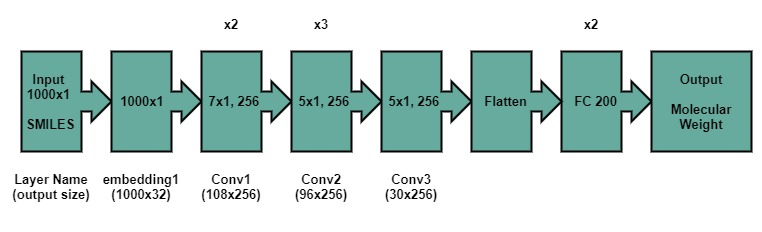
\includegraphics[width=0.5\textwidth]{figures/MW-model_arquitecture.jpg}
        \caption{The architecture of the model that predicts the molecular weight of a compound based on its SMILES string.}
        \label{fig:mw-architecture}
    \end{figure}
    \begin{figure}
        \centering
        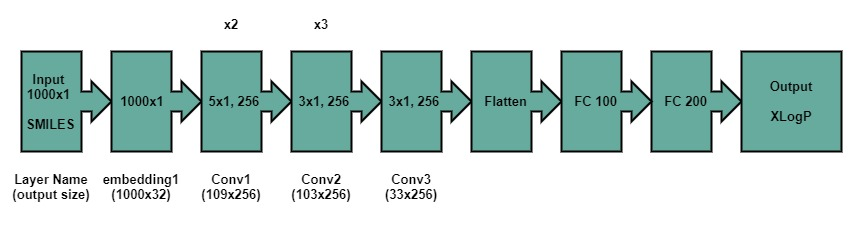
\includegraphics[width=0.5\textwidth]{figures/XLogP-model_arquitecture.jpg}
        \caption{The architecture of the model that predicts the XLogP of a compound based on its SMILES string.}
        \label{fig:xlogp-archi1}
    \end{figure}
    \begin{figure}
        \centering
        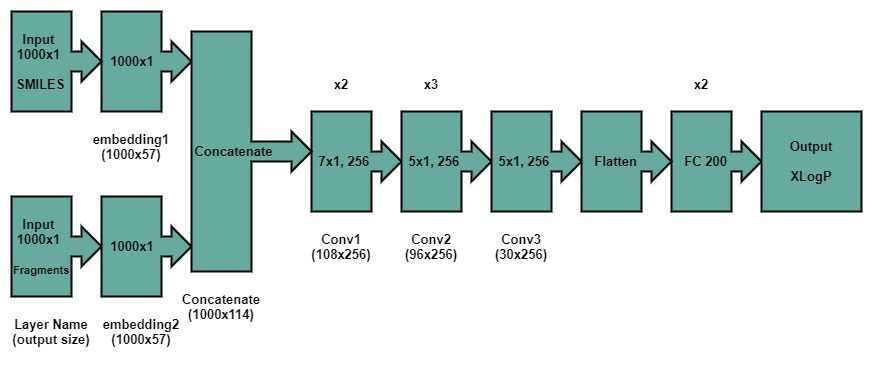
\includegraphics[width=0.5\textwidth]{figures/XLogP_frag_model_arquitecture.jpg}
        \caption{The architecture of the model that predicts the XLogP of a compound based on its SMILES string and RECAP fragments.}
        \label{fig:model23-mol-weight-loss}
    \end{figure}

\graphicspath{ {./figures/} }
\section{Experiments \label{experiments}}
    \subsection{Environment}
        \begin{itemize}
            \item Python 3.8 was the language used for developing the machine learning models. 
            \item The libraries used to implement the models were Tensorflow 2.4, Keras, and Jupyter Notebook to help with the visualization.
            \item The models were trained on a Dell Poweredge R940XA Server that had 2 Intel Xeon Gold 5122 processors, 256GB of RAM, 2 NVIDIA Tesla V100 32G Passive GPU, and a 2TB HDD.
            \item The server ran a Docker container with the Ubuntu 18.04.4 LTS OS.
        \end{itemize}
    \subsection{Datasets}
        \begin{itemize}
            \item The data used for training the models were obtained from the PubChem database (REF).
            \item Using the PubChem REST API we were able to generate a dataset of $\sim$1.33 million entries.
            \item These entries were randomly chosen from the database.
            \item Each entry contained the following information: CID (the unique identifier used by PubChem), molecular formula, canonical SMILES, isometric SMILES, molecular weight, XLogP, exact mass, TPSA, complexity.
            \item For training all the models the canonical SMILES were used as input and for the third model fragments were used as well.
            \item The canonical SMILES was preferred since it gave us enough information about the molecular structure and helped ensure that each compound had a unique SMILES string.
            \item Most of the SMILES strings had a length of less than 200, with the average length being around 56.
            \item Since the SMILES consisted of the symbols of the elements and special characters with no white-space, instead of sentences, we considered more effective to tokenize the strings at character level before being given as input to the model. 
            \item It was then converted into a vector and given padding to ensure they all had the same length.
            \item The fragments used as input were generated using the RECAP technique.
            \item Fragments are similar to SMILES string, but instead represent the compound as a set of smaller SMILES strings.
            \item To generate the fragments we used the RDKit \cite{rdkit} Python library.
            \item When generated they were stored as a string where each fragment was separated by a white-space.
            \item Since not all of the compounds generated a set of fragments, then when not available the SMILES string was used instead. Acting as a single fragment.
            \item These fragment strings were processed the same way as the SMILES strings.
            \item They were tokenized at a character level, vectorized, and given a padding.
            \item The molecular weight and XLogP of the compounds were also important as they were necessary to establish how good predictions of the models were.
            \item The molecular weights from the dataset ranged from $\sim$1 to $\sim$10,000 g/mol, with the average being at $\sim$439.44 g/mol.
            \item The XLogP from the dataset ranged from $\sim$-70 to $\sim$161, with the average being at $\sim$4.58.
            \item The dataset was split into 3 subsets: training, validation, and test sets. 
            \item The training set consisted of 600,000 elements of the data and was used for training the model.
            \item The validation set consisted of 200,000 elements of the data and was used while training to help fit the hyperparameters of the model.
            \item Finally, the test set consisted of 200,000 elements of the data was used to evaluated the model after training.
            \item The data that was not used was saved for any further testing we might want to do on the model.
        \end{itemize}
    
    % Figures
    \begin{figure}
        \centering
        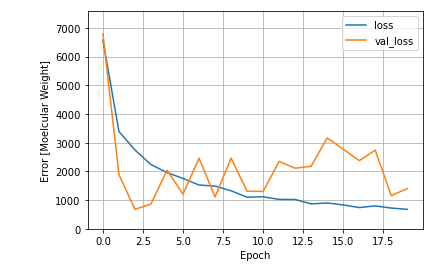
\includegraphics[width=0.5\textwidth]{loss_gragh_20_epoch.PNG}
        \caption{The loss graph of the first trained model for predicting molecular weight.}
        \label{fig:model2-mol-weight-loss}
    \end{figure}
    \begin{figure}
        \centering
        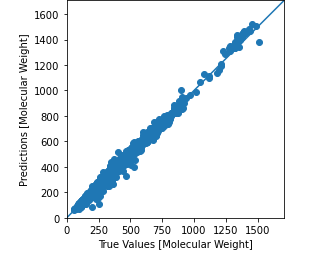
\includegraphics[width=0.5\textwidth]{model_2_prediction.PNG}
        \caption{Results of the first trained model for predicting molecular weight.}
        \label{fig:model2-mol-weight-predictions}
    \end{figure}
    \begin{figure}
        \centering
        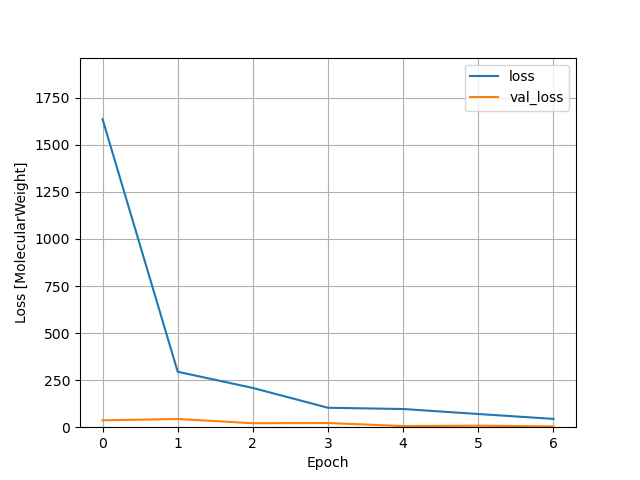
\includegraphics[width=0.5\textwidth]{model_23_7_epochs_loss_MolecularWeight.png}
        \caption{Loss graph of the latest tuned model for predicting molecular weight.}
        \label{fig:model23-mol-weight-loss}
    \end{figure}
    \begin{figure}
        \centering
        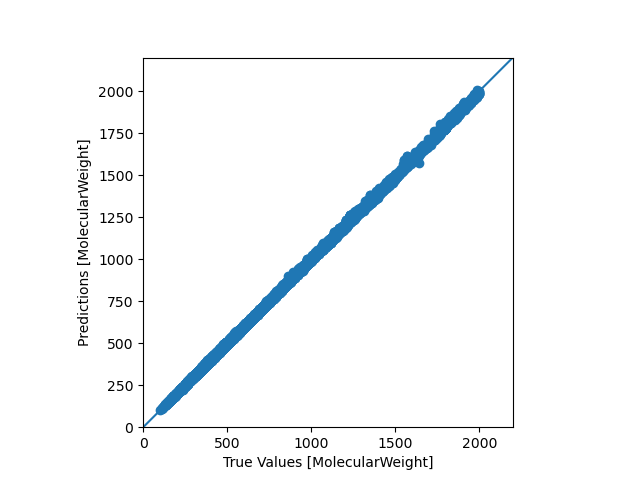
\includegraphics[width=0.5\textwidth]{model_23_7_epochs_predictions_MolecularWeight.png}
        \caption{Results latest tuned model for predicting molecular weight.}
        \label{fig:model23-mol-weight-predictions}
    \end{figure}
    \begin{figure}
        \centering
        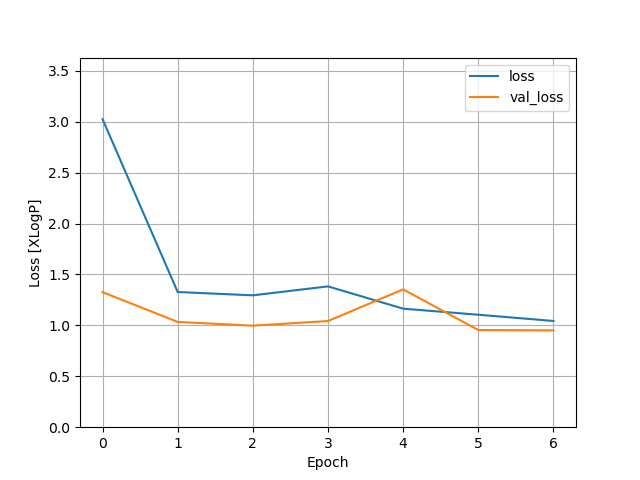
\includegraphics[width=0.5\textwidth]{model_7_7_epochs_loss_XLogP.png}
        \caption{Loss graph of the first trained model for predicting XLogP.}
        \label{fig:model7-xlogp-loss}
    \end{figure}
    \begin{figure}
        \centering
        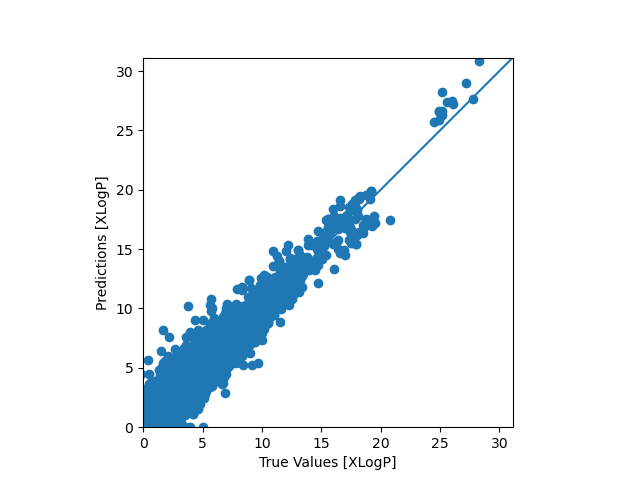
\includegraphics[width=0.5\textwidth]{model_7_7_epochs_predictions_XLogP.png}
        \caption{Results of the first trained model for predicting XLogP.}
        \label{fig:model7-xlogp-predictions}
    \end{figure}


\section{Related Works \label{relwork}}

\section{Conclusions \label{conclude}}


\section*{Acknowledgements}
This work was supported by the Center for the Advancement of Wearable Technologies and the National Science Foundation under  grant OIA-1849243. 
%Any opinions, findings, and conclusions or recommendations expressed in this material are those of the author(s) and do not necessarily reflect the views of the National Science Foundation.


{\footnotesize
\bibliography{references}
\bibliographystyle{ieeetr}
}

\end{document}